\section{The Compact Muon Solenoid}
\label{sec:CMS}
At one of the collision points of the LHC, the CMS detector\cite{CMS, Bayatian:2006zz,Bayatian:922757} is placed. Weighing 14 000~\tonne, this cylindrical detector is about 28.7~\meter\ long and 15~\meter\ in diameter. It has an onion like structure of several specialised detectors and contains a superconducting solenoid with a magnetic field of 3.8~\Tesla. Living in a hadronic environment, multi-jet processes produced by the strong interaction are a main source of background for rare physics processes. Therefore, good identification, momentum resolution, and charge determination of muons, electrons and photons are one of the main goals of the CMS detector. Additionally, a good charged particle momentum resolution and reconstruction efficiency in the inner tracker provides identification for jets coming from \Pbottom\ quarks or tau particles can be identified. Also the electromagnetic resolution for an efficient photon and lepton isolation as well as a good hadronic calorimeter for the missing transverse energy\footnote{The missing transverse energy comes from an imbalance in the transverse plane. This will be discussed in Chapter 4.} were kept into account while designing CMS. In \fig{fig:CMS}, an overview of the CMS detector is shown. 
\begin{figure}[htbp]
	\centering
	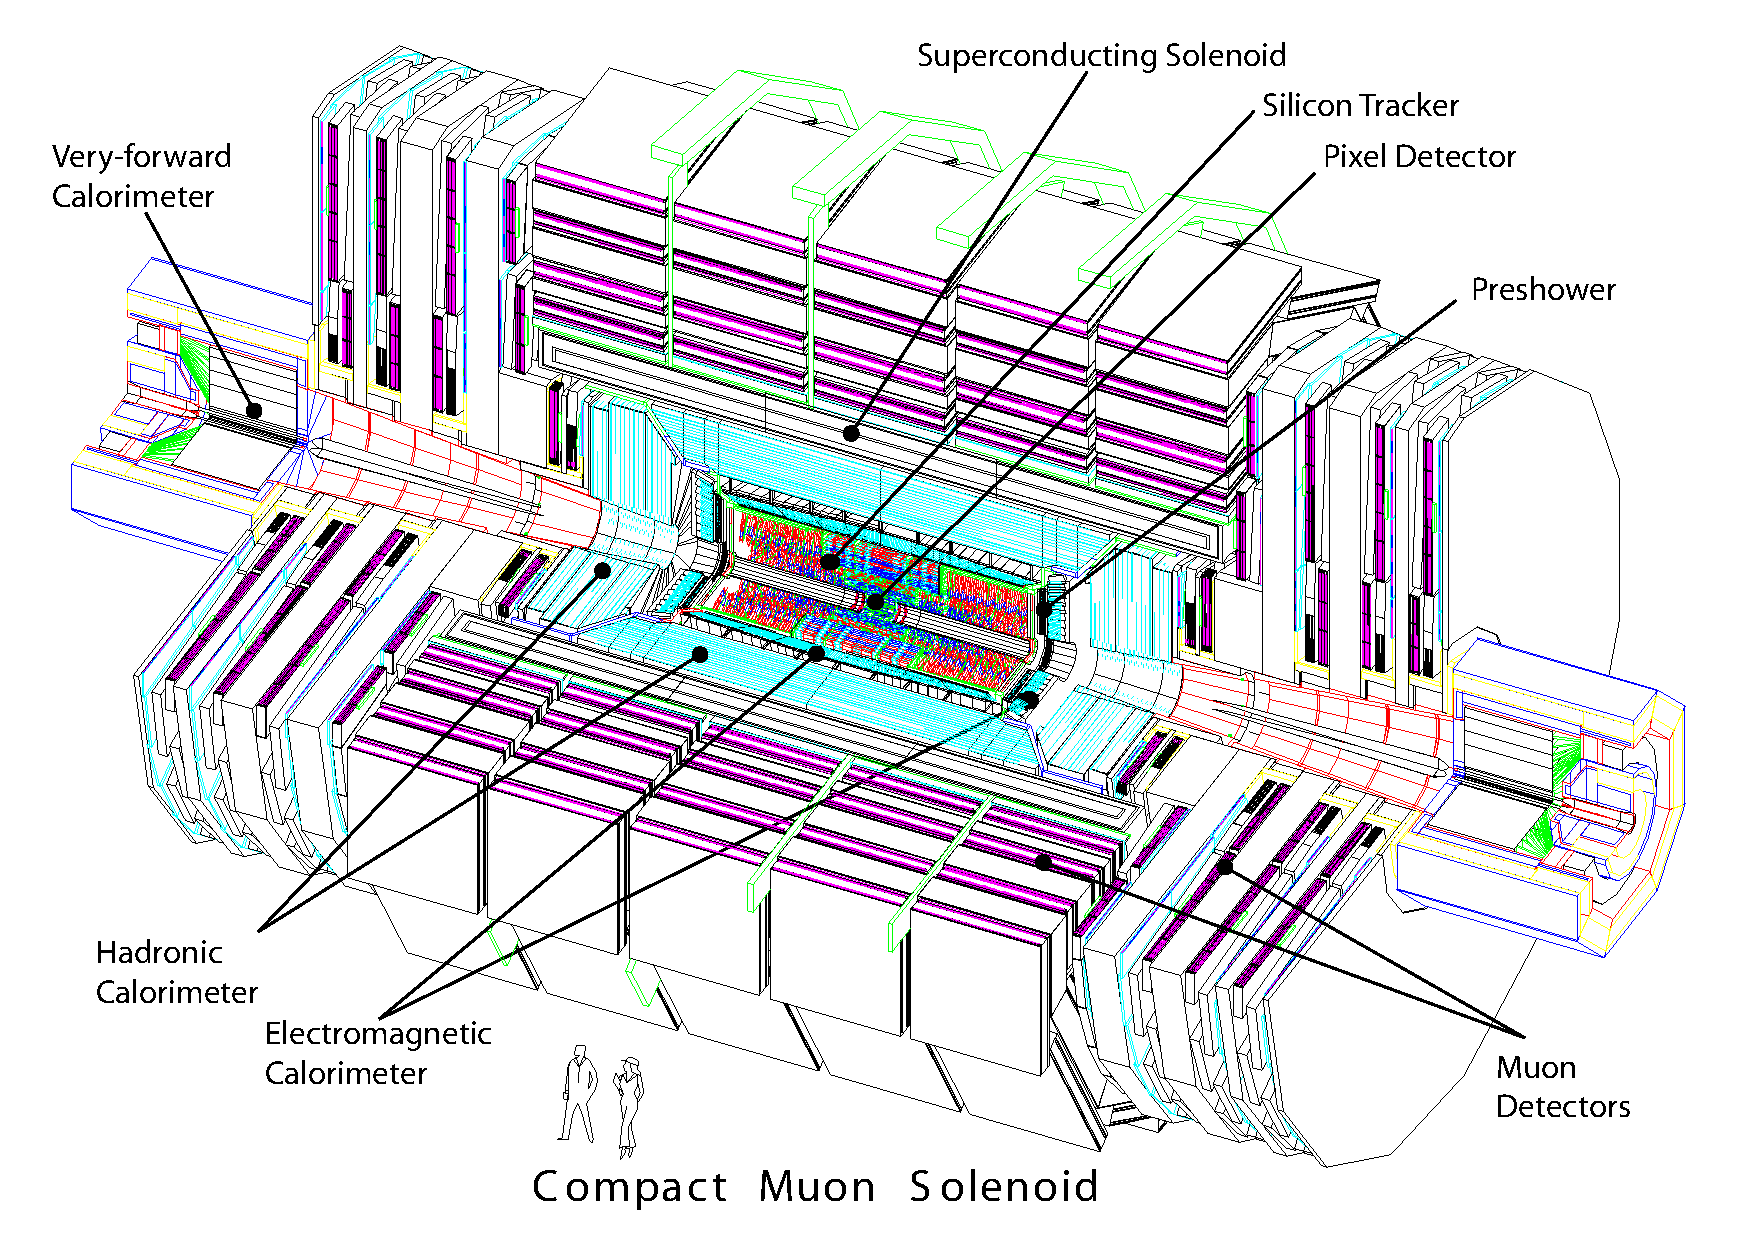
\includegraphics[width=\textwidth]{2_ExperimentalSetup/Figures/cms_complete_labelled}
	\caption{Mechanical layout of the CMS detector. Figure taken from~\cite{CMSdraw}.}
	\label{fig:CMS}
\end{figure}

\subsection{CMS coordinate system}
The coordinate system used by CMS can be found in \fig{fig:CMScoord}. The origin of the right handed orthogonal coordinate system is chosen to be the point of collisions. The x-axis points towards the centre of the LHC ring such that the y-axis points towards the sky, and the z-axis lies tangent to the beam axis. Since the experiment has a cylindrical shape, customary coordinates are used to describe the momentum \impuls: the distance $p=|\vec{p}|$, the azimuthal angle\footnote{The azimuthal angle is the angle between the x-axis and the projection in the transverse plane of the momentum \impuls, denoted as \trimpuls. } $\phi \in \left[-\pi,\pi\right]$, the pseudo-rapidity\footnote{The pseudo rapidity  is expressed by the polar angle $\theta$ between the direction of \impuls and the beam.} \psrap: 
\begin{equation}
\eta = - \ln \left(\tan \left(\frac{\theta}{2}\right)\right).
\end{equation}
For the energies considered at the LHC, where $E >> m$, the pseudo-rapidity is a good approximation of the rapidity $y$
\begin{equation}
y = \frac{1}{2} \ln \left(\frac{E + p_z}{E - p_z}\right), 
\end{equation}
where the difference of rapidities of two particles is invariant under a Lorentz boost in the z-direction.
 \begin{figure}[htbp]
	\centering
	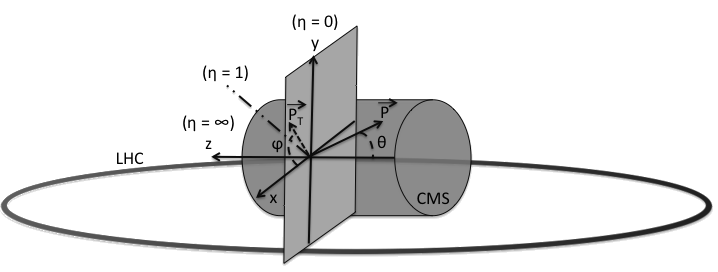
\includegraphics[width=1.\textwidth]{2_ExperimentalSetup/Figures/imageedit_1_9146672677}
	\caption{Representation of the coordinate system used by CMS. The point of origin is put at the collision point. The x-axis points towards the centre of the LHC ring such that the z-axis lies tangent to the beam axis. }
	\label{fig:CMScoord}
\end{figure}

\subsection{Towards the heart of CMS}
The CMS detector can be divided into two parts. A central barrel is placed around the beam pipe $ \left(\abspsrap <1.4\right)$, and two plugs (end caps) ensure the hermeticity of the detector. In \fig{fig:CMS} and \fig{fig:CMSview} the onion like structure of the CMS detector is visible. The choice of a solenoid of 12.9 \si{ \meter}  long and 5.9 \si{ \meter}
diameter gives the advantage of bending the particle trajectories in the transverse plane. The hadronic calorimeter (\Sec{sec:HCAL}),  the electromagnetic calorimeter (\Sec{sec:ECAL}) and the tracker (\Sec{sec:TRK}) are within the solenoid (\Sec{sec:SOL}), while the muon chambers (\Sec{sec:MUO}) are placed outside the solenoid. The data used for the search presented in this thesis is collected after the long shutdown 1. After discussing each part of CMS in their Run 1 configuration, \Sec{sec:Phase1} elaborates on their different upgrades for the data collected in Run 2. 
\begin{figure}[htbp]
	\centering
	\includegraphics[width=1.\linewidth]{2_ExperimentalSetup/Figures/cmsview1}
	\includegraphics[width=1.\linewidth]{2_ExperimentalSetup/Figures/cmsview}
 \caption{Schematic view of the CMS detector in the Run I configuration. The longitudinal view of one quarter of the detector is given on top, while the transversal view is shown on the bottom. The muon system barrel elements are denoted as MBZ/N/S, where z$=-2...+2$ is the barrel wheel number, n$=1...4$ the station number and S$=1...12$ the sector number. Similary, the steel return yokes are denoted as YBZ/N/S. The solenoid is denoted as CB0, while the hadronic calorimeter is denoted as HE (end cap)/ HB (barrel)/HF (forward) and the electromagnet calorimeter as EE (end cap)/EB (barrel). The green part represents the tracking system (tracker + pixel). Figure taken from~\cite{Chatrchyan:1223944}}.
	\label{fig:CMSview}
\end{figure}

\clearpage
\subsubsection{Muon system}
\label{sec:MUO}
% PHOTO https://cds.cern.ch/record/2016943
% and http://cms.web.cern.ch/news/news-point-5-22-november-2013
The outermost part of CMS consists of the muon system. The magnet return yoke is interleaved with gaseous detector chambers for muon identification and momentum measurement. The barrel contains muon stations arranged in five separate iron wheels, while in the end cap four muon stations are mounted onto three independent iron discs on each side. Each barrel wheel has 12 sectors in the azimuthal angle. 

The muon system is divided into three parts, shown in \fig{fig:muonsys}. The muon rate and neutron induced backgrounds are small and the magnetic field is very low for the barrel, thus CMS can use drift tube (DT) chambers. For the end caps however, the muon and background flux is much higher and there is a need to use cathode strip chambers (CSC) which are able to provide a faster response, higher granularity and have a better resistance against radiation. In order to form a redundant trigger system, resistive plate chambers (RPC) are added. This makes a total of 250 DT, 540 CSC and 610 RPC chambers. In \fig{fig:CMSview} the arrangement is shown.
\begin{figure}[htbp]
	\centering
	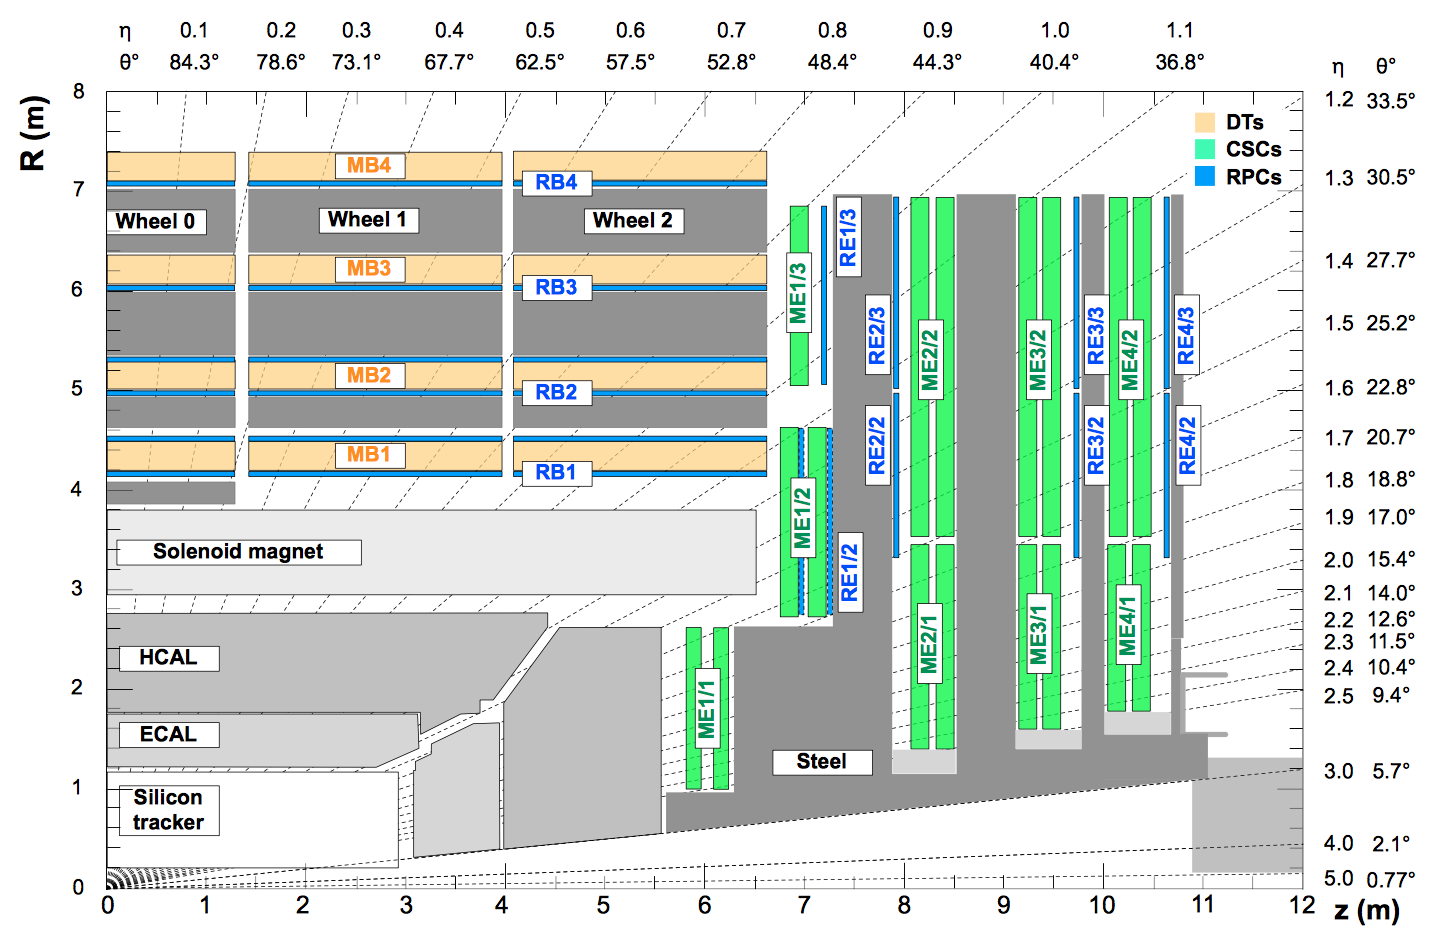
\includegraphics[width=.69\textwidth]{2_ExperimentalSetup/Figures/muonsys}
	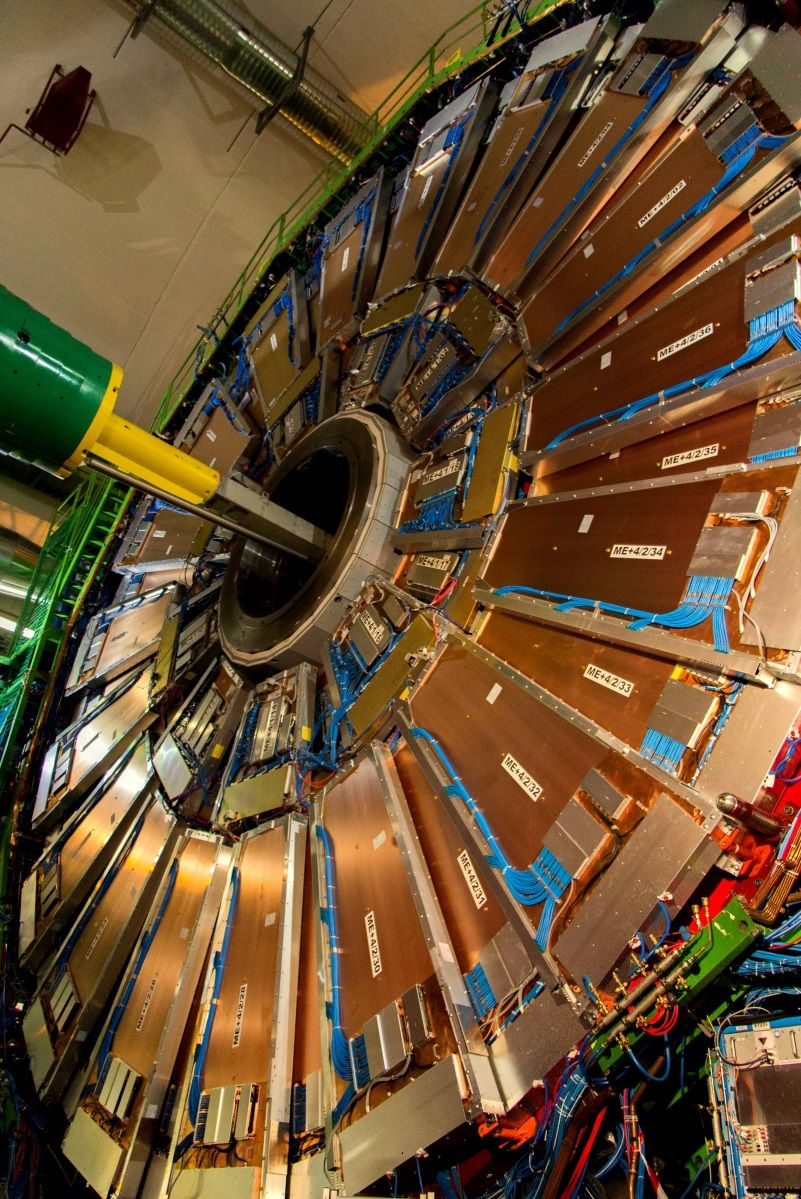
\includegraphics[width=0.3\linewidth]{2_ExperimentalSetup/Figures/NfP5131122image6}
	\caption{(Left) Schematic view of one quarter of the CMS muon system in the Run I configuration. The cathode strip chambers (CSC) are shown in green, the drift tubes (DT) are shown in yellow, while the resistive plate chambers (RPC) are shown in blue. Figure  taken from \cite{Chatrchyan:1223944}. (Right) Cathode strip chambers (ME+4/2 chambers on YE+3). Photo taken from \cite{muon}.}
	\label{fig:muonsys}
\end{figure}


Providing a measurement for \abspsrap $<1.2$, the DT chambers in the barrel are on average $2 \times 2.5\:\meter^2$ in size and consist of 12 layers of DT cells\footnote{The DT cells are 4~\centi \meter\ wide gas tubes with positively charged stretched wires inside.} arranged in three groups of four. The $r\phi$ coordinate is provided by the two outside groups, while the middle group measures the $z$ coordinate. %For each $\phi$ sector, the DT chamber is mixed with the flux return yoke. 
For the outer muon station, the DT chambers contain only 8 layers of DT cells, providing a muon position in th $r\phi$ plane.
There are four CSC stations in each end cap, providing muon measurements for $0.9<$ \abspsrap $<2.4$ (Run I configuration). These CSCs are multi-wired proportional chambers that consist of 6 anode wire planes crossed by 7 copper strips cathode panels in a gas volume. The $r$ coordinate is provided by the copper strips, while the $\phi$ coordinate comes from the anode wires, giving a two dimensional position measurement. 
There are six layers of RPCs in the barrel muon system and one layer into each of the first three stations of the end cap. They are made from two high resistive plastic plates with an applied voltage and separated by a gas volume. Read out strips mounted on top of the plastic plates detect the signal generated by a muon passing through the gas volume. The RPCs provide a fast response with a time resolution of 1~\nano \second\ and cover a range of \abspsrap $<1.8$ for the Run 1 configuration. 

The muon system provides triggering on muons, identifying muons and improves the momentum measurement and charge determination of high $p_T$ muons. On top of the muon system, the muon energy is deposited in the electromagnetic calorimeter, the hadronic calorimeter, and outer calorimeter. 
%(FIXME not tracker? heel licht tov calos, gemaakt om deeltjes niet te hinderen, calos wel) 
The high magnetic field enables an efficient first level trigger and allows a good momentum resolution of $\Delta p / p \approx 1\%$ for a $p_T$ of 100~\GeV\ and $\approx 10\%$ for a $p_T$ of 1~\TeV \todo{check numbers for run 2}. There is an efficient muon measurement up to \abspsrap $<2.4$.

\subsubsection{Solenoid}
\label{sec:SOL}
	Making use of the knowledge of previous experiments like ALEPH and DELPHI at LEP and H1 at HERA, CMS choose for a large super conducting solenoid with a a length of 12.9~\meter\ and a inner bore of 5.9~\meter~\cite{Bayatian:922757}. With 2 168 turns, a current of 19.5~\kilo \ampere\ and  a total energy of 2.7~\giga \joule, a large bending power can be obtained for a modestly-sized solenoid. In order to ensure a good momentum resolution in the forward regions, a favourable length/radius was necessary.  In \fig{fig:CMSsolenoid}, a photo of the CMS solenoid is shown. 

	The solenoid uses a high-purity aluminium stabilised conductor with indirect cooling from liquid helium, together with fully epoxy impregnation. A four-layer winding is implemented that can withstand an outward pressure of 64 \si{ \atm}. The NbTi cable is co-extruded by pure aluminium that acts as a thermal stabilizer and has an aluminium alloy for mechanical reinforcement. The return of the magnetic field is done by fives wheels, noted by YB in \fig{fig:CMSview}.
	\begin{figure}[htbp]
		\centering
		\begin{minipage}{0.6\textwidth}
		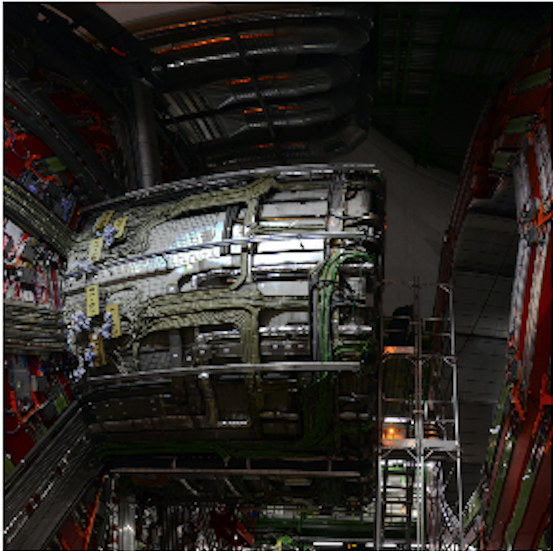
\includegraphics[width=1.\textwidth]{2_ExperimentalSetup/Figures/solenoid.png}
	\end{minipage}
		\begin{minipage}{0.39\textwidth}
		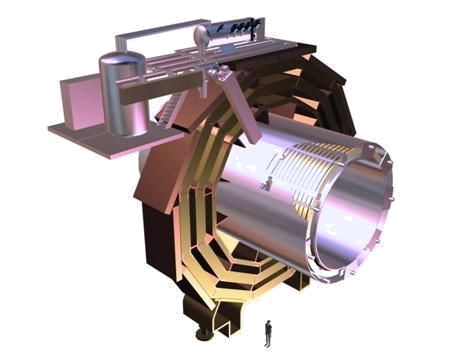
\includegraphics[width=\textwidth]{2_ExperimentalSetup/Figures/839_1a}
		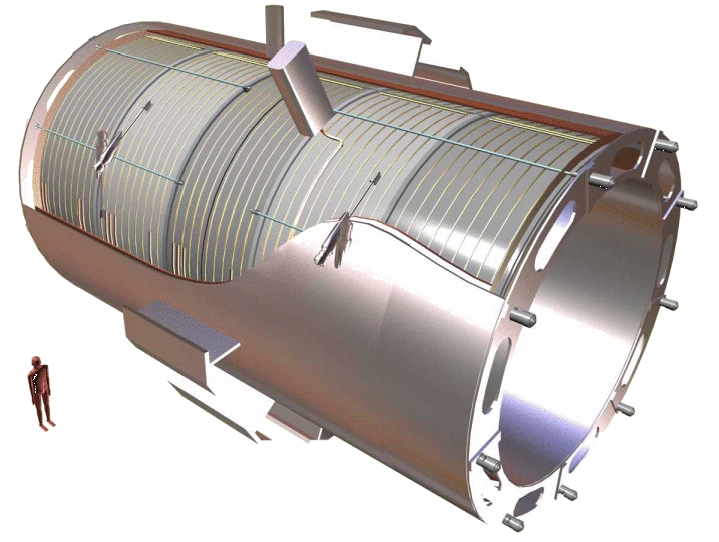
\includegraphics[width=\textwidth]{2_ExperimentalSetup/Figures/CMS-solenoid-magneta}
	\end{minipage}
		\caption{(Left) CMS solenoid during the long shutdown in 2013. (Right) An impression of the solenoid magnet taken from \cite{solenoid}.}
	%http://slideplayer.com/slide/10648021/
	
		\label{fig:CMSsolenoid}
	\end{figure}	
	
\subsubsection{Hadronic calorimeter}
\label{sec:HCAL}
% PHOTO http://cms.web.cern.ch/news/cms-prepares-pixel-and-hcal-upgrades
% http://cds.cern.ch/record/2235509?ln=en peformance
%http://home.fnal.gov/~chlebana/CMS/Phase2/LPCPhase2Simulation/notes/NOTE2006_138-1.pdf
%http://physics.bu.edu/neppsr/2006/TALKS-2006/Calorimetry_Surrow.pdf
The hadronic calorimeter (HCAL) is dedicated to precisely measure the energy of charged and neutral hadrons via a succession of absorbers and scintillators. This makes it crucial for physics analyses with hadronic jets or missing transverse energy. The HCAL barrel extends between 1.77 $<r<$ 2.95~\meter, where $r$ is the radius in the transverse plane with respect to the beam. Due to space limitations, the HCAL needs to be as small as possible and is made from materials with short interaction lengths\footnote{Here the interaction length is the nuclear interaction length and this is the length needed for absorbing 36.7\% of the relativistic charged particles. For the electromagnetic calorimeter this is defined in radiation length $X_0$. The radiation length is the mean distance over which a high energy electron loses all but $1/e$ of its energy by bremsstrahlung.}. 
On top of this, the HCAL should be as hermetic as possible and extend to large absolute pseudo rapidities such that it can proved a good measurement of the missing transverse energy. 

The quality of the energy measurements is dependent on the fraction of the hadronic shower that can be detected. Therefore, the HCAL barrel (HB) inside the solenoid is reinforced by an outer hadronic calorimeter between the solenoid and muon detectors (HO, see \fig{fig:HCAL}), using the solenoid as extra absorber. This increases the thickness to 12 interaction lengths.  The HB and HO provide measurements for $\abspsrap<1.3$, while an end cap on each side (HE, $1.3< \abspsrap <3$) and a forward calorimeter (HF, $3.0< \abspsrap < 5.2$) extend the pseudo rapidity range. 


\begin{figure}[htbp]
	\centering
	%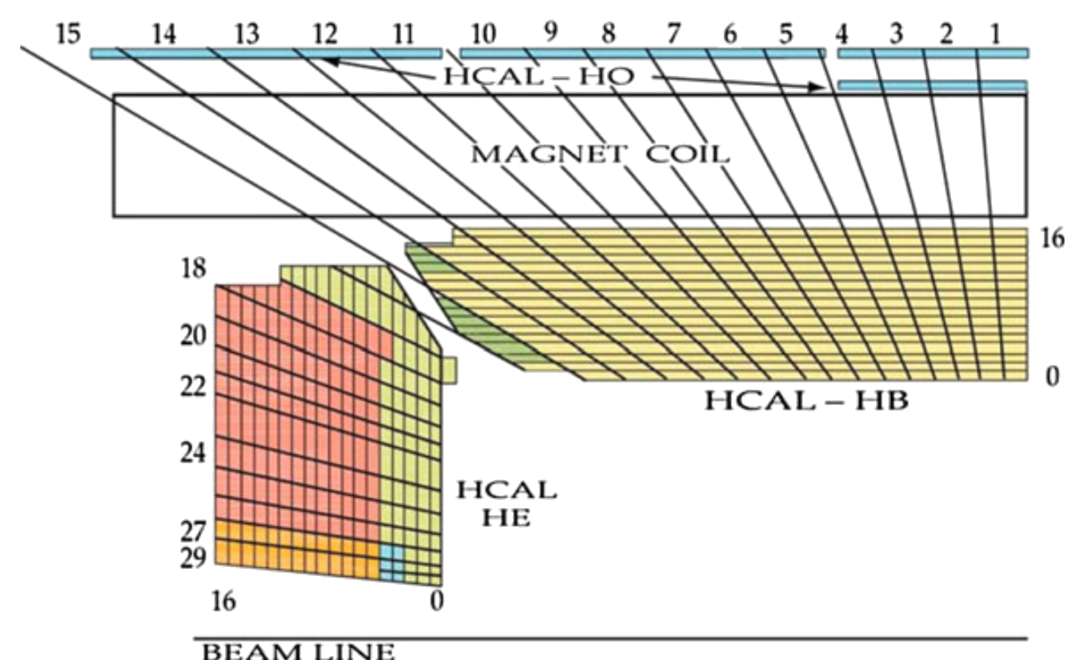
\includegraphics[width=0.59\textwidth]{2_ExperimentalSetup/Figures/imageedit_12_3242046754}hcalquarter
	%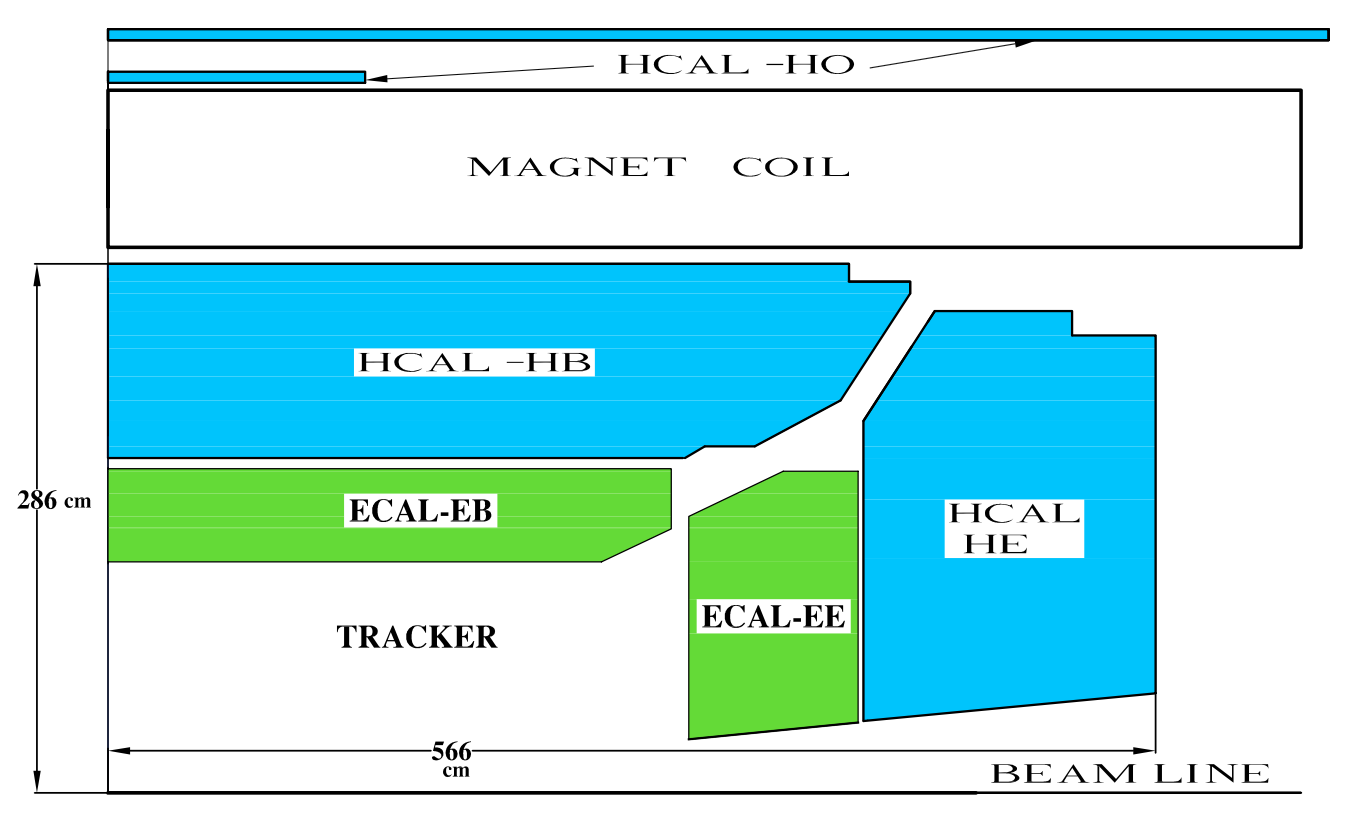
\includegraphics[width=0.59\textwidth]{2_ExperimentalSetup/Figures/hcalquarter}
	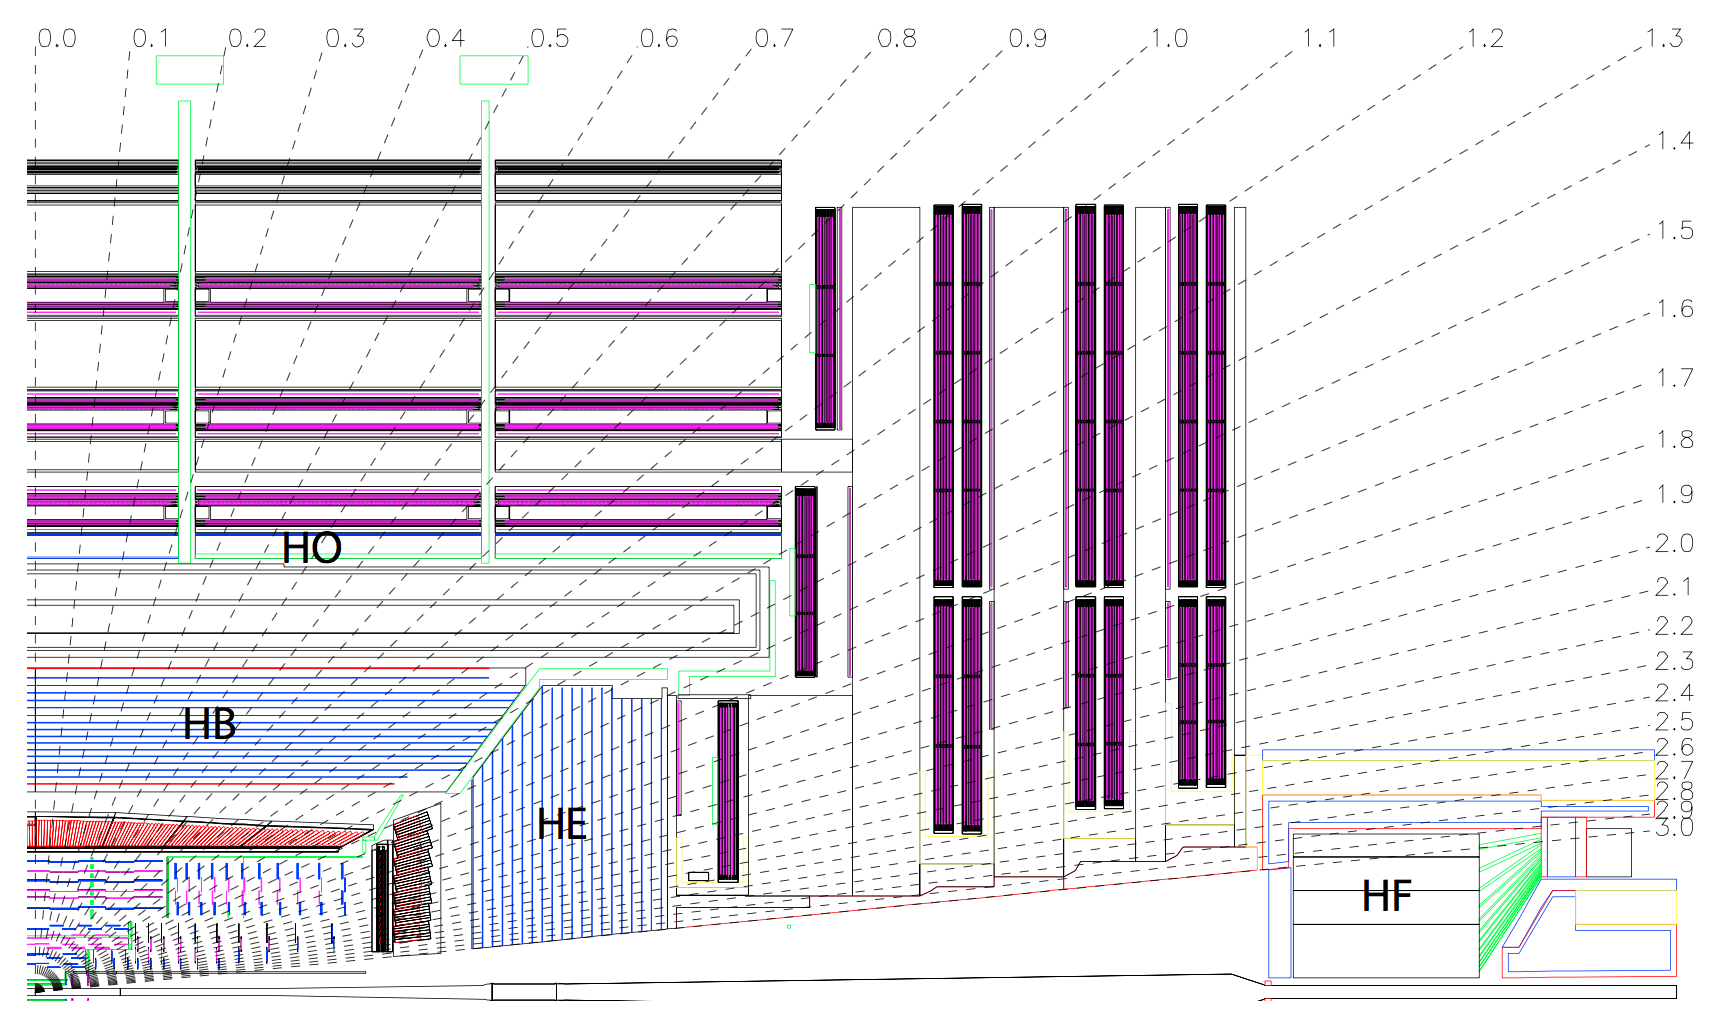
\includegraphics[width=0.6\textwidth]{2_ExperimentalSetup/Figures/HCAL2}
		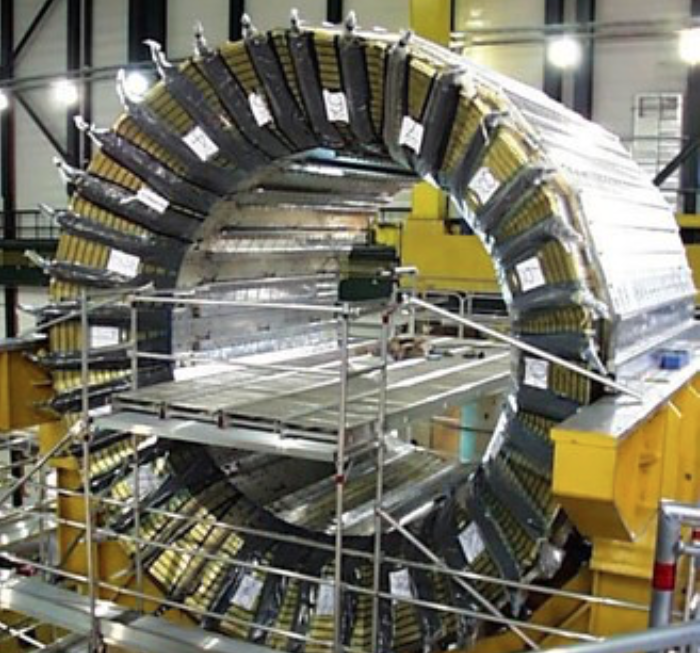
\includegraphics[width=0.\textwidth]{2_ExperimentalSetup/Figures/HCAL}
	%\caption{(Left) Tower segmentation for one quarter of the HCAL displayed in the $rz$ plane. Figure taken from \cite{Chatrchyan:2008aa}. (Right) CMS barrel calorimeter. Photo taken from \cite{HCAL}.}
 %\caption{(Left) Location of the HCAL detectors (blue) displayed in the $rz$ plane. Figure taken from \cite{Baiatian:1049915}. (Right) CMS barrel calorimeter. Photo taken from \cite{HCAL}.}
 \caption{(Left) Longitudinal view of the CMS detector showing the locations of the HB, HE, HO, and HF calorimeters. Figure taken from \cite{Chatrchyan:2008aa}. (Right) CMS barrel calorimeter. Photo taken from \cite{HCAL}.}
	\label{fig:HCAL}
\end{figure}

The HB is made of 16 absorber plates where most of them are built from brass and others are made from stainless steal and is about five to ten interaction lengths thick. It is divided in $\eta \times \phi$ towers and contains 2592 read out channels. The HO complements the HB and extends the reach up to twelve interaction lengths. This subsystem contains 2160 read out channels. The HE is also composed of brass absorber plates and has a thickness corresponding to approximately ten interaction lengths, with 2592 read out channels.. 
The HF experiences intense particle fluxes with an expected energy of 760~\GeV\ deposited on average in a proton interaction at a centre-of-mass of 14~\TeV, compared to 100~\GeV\ in the rest of the detector. Therefore, these are Cherenkov light detectors made of radiation hard quartz fibers.
The main causes of such large energy events are high energy muons, cosmic particles and charged particles from late showering hadrons. During  Run 1, it became clear that the glass windows of the photon multiplier tubes (PMTs) had to be replaced which was done during LS1~\cite{Tiras:2016ghv}. The HF represents 1728 read out channels. 

The HCAL and electromagnetic calorimeter combined can measure the hadron energy with a resolution $\Delta E /E \approx 100\% \sqrt{E[\GeV]} + 5\%$. 	
\subsubsection{Electromagnetic calorimeter}
\label{sec:ECAL}
The electromagnetic calorimeter (ECAL) is designed to measure the energy of photons and electrons and covers \abspsrap $<3$. It is an hermetic, homogeneous detector and consists of 75 848 lead tungstate (PbW$O_4$) crystals. These crystals have a fast response time - 80\% of the light is emitted within 25 \si{ \nano \second} - and are radiation hard. The electromagnetic showers produced by passing electrons or photons ionize the crystal atoms which emit a blue-green scintillation light, that is collected by silicon avalanche photodiodes (APDs) in the barrel and vacuum phototriodes (VPTs) in the end caps. The crystals and the APD response is sensitive to temperature changes and require a stable temperature. 

\begin{figure}[htbp]
	\centering
	\begin{minipage}{0.5\textwidth}
		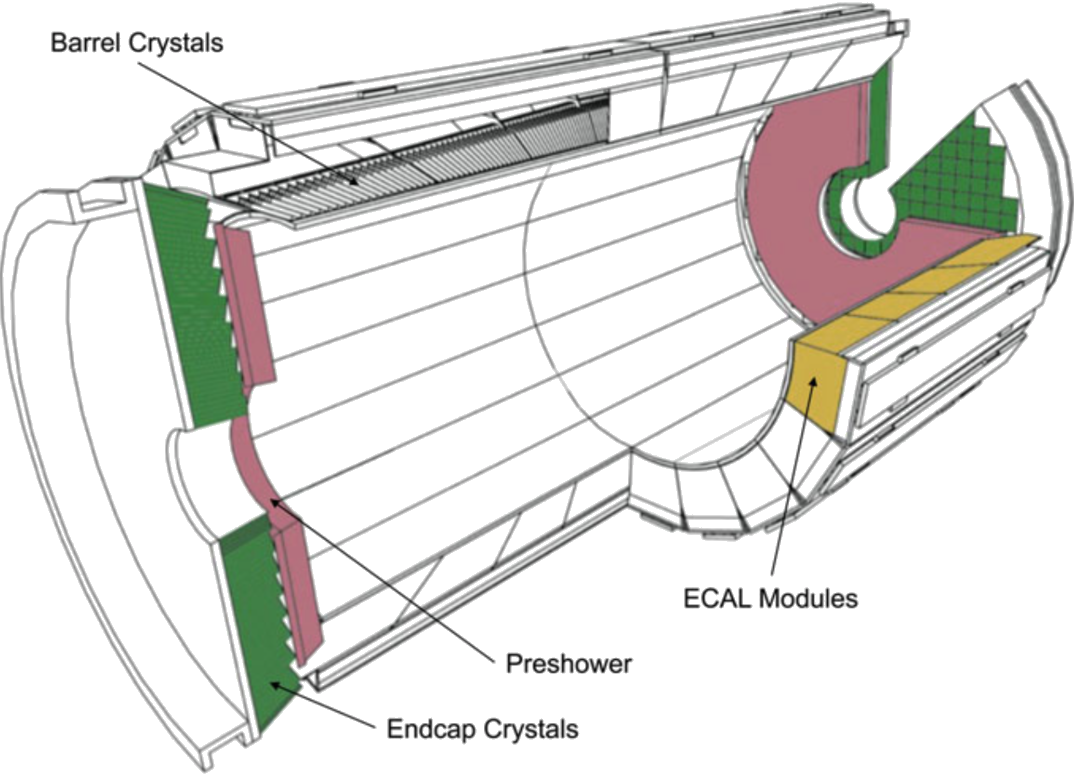
\includegraphics[width=\textwidth]{2_ExperimentalSetup/Figures/imageedit_5_8264930617}
	\end{minipage}
\begin{minipage}{0.39\textwidth}
	\includegraphics[width=\textwidth]{2_ExperimentalSetup/Figures/ECAL}
	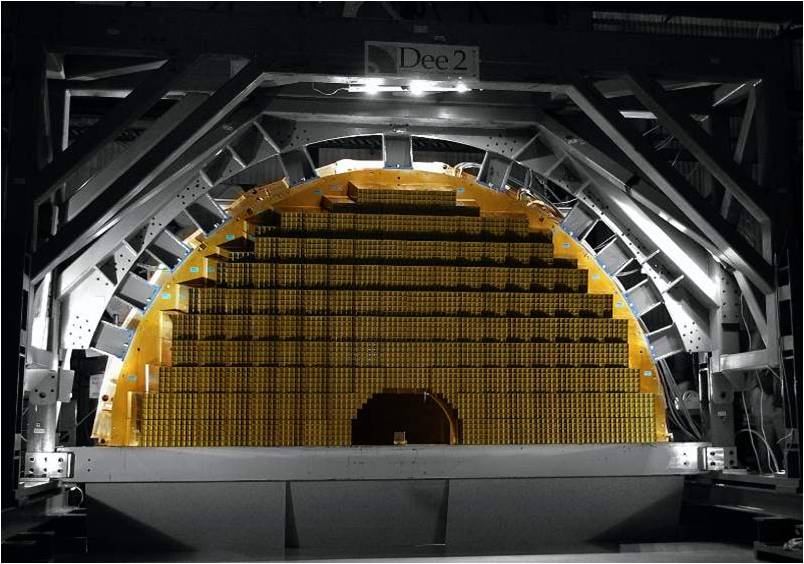
\includegraphics[width=\textwidth]{2_ExperimentalSetup/Figures/EE-in-frame}
	%http://slideplayer.com/slide/8696989/
\end{minipage}
	\caption{(Left) Schematic cross section of the electromagnetic calorimeter taken from \cite{Chatrchyan:2008aa}. (Right top) The ECAL barrel during construction~\cite{ECAL}. (Right bottom) One half of an EE~\cite{EE}.}
	\label{fig:ECAL}
\end{figure}
There are three regions: a central barrel (EB), an endcap region (EE) and a preshower (ES) (\fig{fig:ECAL}). 
The EB has an inner radius of 129~\centi \meter\ and corresponds to a pseudo rapidity of $0 < $ \abspsrap $<1.479$. At a distance of 314~\centi \meter\ from the vertex and covering a pseudo rapidity of $1.479 < $ \abspsrap $<3.0$, are the EE. They consist of semi-circular aluminium plates from which structural units of $5\times5$ crystals (super crystals) are supported. The ES is placed in front of the crystal calorimeter over the end cap pseudo rapidity range with two planes of silicon strip detectors as active elements. 

The electromagnetic shower will typically involve more than one channel. More than 90\% of the energy of a 35~\GeV\ electron or photon is contained in a $5\times 5$ matrix of crystals. Therefore, a clustering algorithm is performed in order to associate the energy deposits to the particles impinging the calorimeter.
The achieved precision~\cite{1748-0221-12-01-C01069} for the barrel is 2.10$^{-3}$ \si{ \rad} in $\phi$ and 10$^{-3}$ in \psrap. For the end caps this is 5.10$^{-3}$~\rad\ in $\phi$ and 2.10$^{-3}$ in \psrap. The energy is reconstructed by a supercluster algorithm, taking into account energy radiated via bremsstrahlung or conversion~\cite{Chatrchyan:2008aa}.  The energy resolution is given by 
\begin{equation}
\frac{\sigma(E)}{E} = \frac{2.8\%}{\sqrt{E}}\oplus \frac{0.128}{E(GeV)} \oplus 0.3\%, 
\end{equation}
in the absence of a magnetic field, where the contributions come from the stochastic, noise and constant terms respectively. The dominating term is the constant term ($E_{shower} \approx 100~\GeV$) and thus the performance is highly dependent on the quality of calibration and monitoring .


\begin{comment}
The relative energy resolution of the ECAL for electrons is between 1.4-3\% in EB and 3-4\% for EE. In Figure \ref{fig:ECALres}, the resolutions for low and high bremsstrahlung electrons are shown. 
\begin{figure}[htbp]
	\centering
	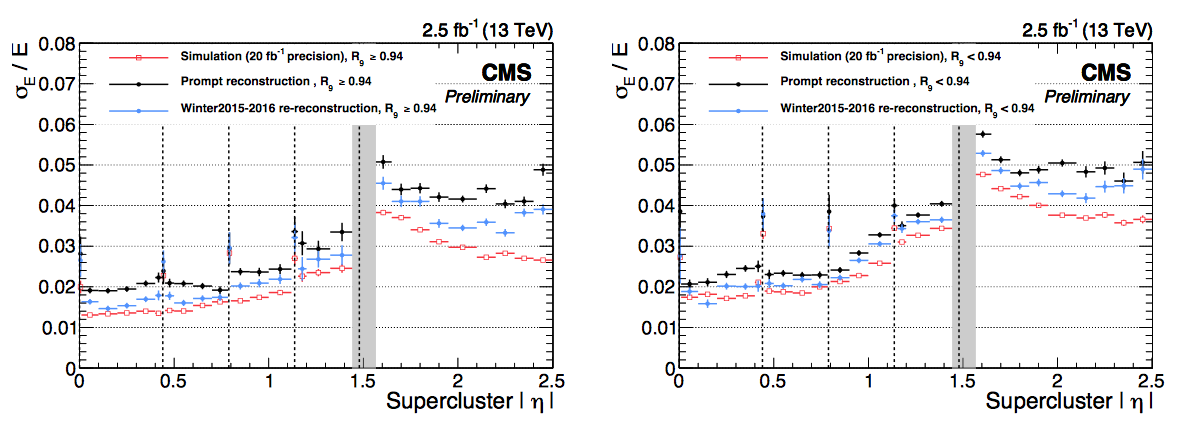
\includegraphics[width=\textwidth]{2_ExperimentalSetup/Figures/imageedit_7_5931623976}
	\caption{Relative energy resolution in bins of pseudo rapidity for the barrel and end caps using electrons from $Z \rightarrow ee$. Left: low bremsstrahlung electrons, Right: high bremsstrahlung electrons\cite{Sun:2233637}.}
	\label{fig:ECALres}
\end{figure}
\end{comment}

\subsubsection{Inner tracking system and operations}
\label{sec:TRK}
% PHOTO https://cds.cern.ch/record/2253519 
%https://indico.cern.ch/event/632928/
%http://cds.cern.ch/search?ln=en&cc=CMS+Reports&sc=1&p=tracker&f=title&action_search=Search
% comparison with atlas https://cds.cern.ch/record/1563583/files/ATL-PHYS-PROC-2013-206.pdf
The tracking system (tracker)~\cite{Chatrchyan:1704291} is the detecting unit closest to the point of interaction. Responsible for the reconstruction of  trajectories from charged particles with \abspsrap $<2.5$ that are bent by the magnetic field, it provides a measurement of the momentum. The tracker is also responsible for the determination of the interaction point or vertex. It should be able to provide high granularity as well as speed, and be able to endure high radiation. For this reason, the CMS collaboration choose silicon detector technology.

\begin{figure}[htbp]
	\centering
%	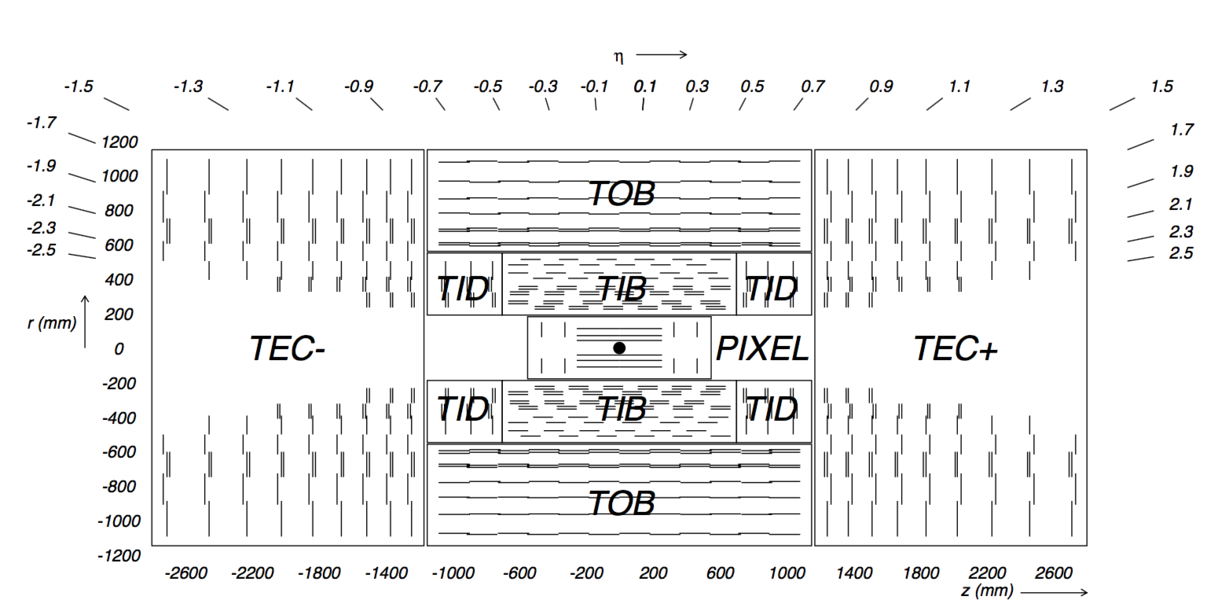
\includegraphics[width=\textwidth]{2_ExperimentalSetup/Figures/imageedit_3_5170744545}
	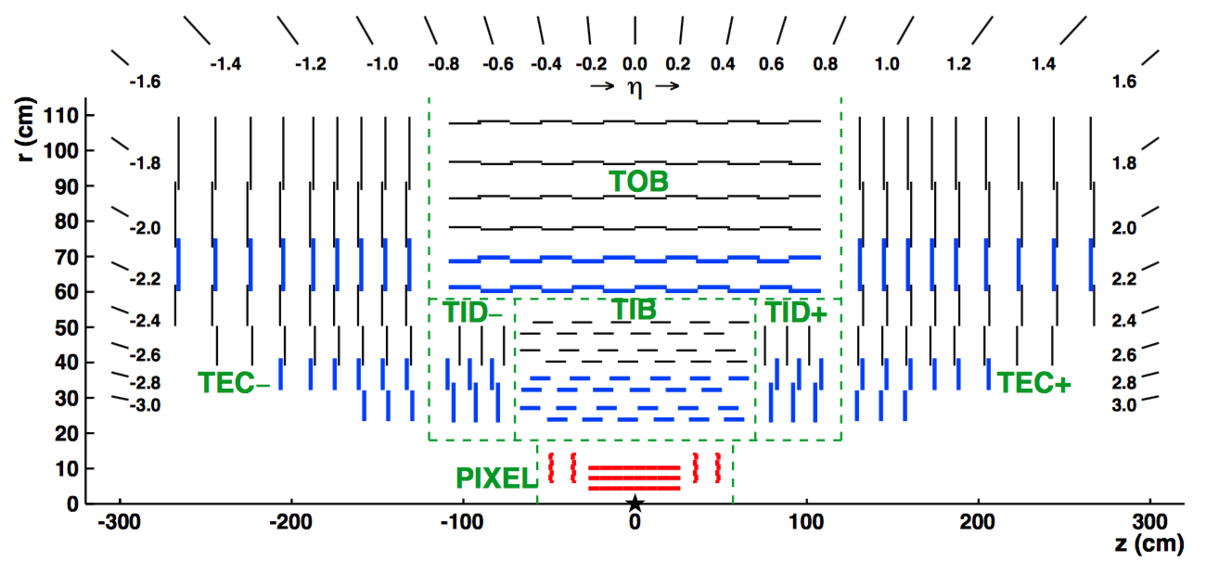
\includegraphics[width=1.\textwidth]{2_ExperimentalSetup/Figures/imageedit_11_9317262269}
%	\caption{Schematic cross section through the CMS tracker. Each line represents a detector module. Double lines indicate back-to-back modules\cite{Chatrchyan:2008aa}.}
  \caption{Schematic cross section of the top half of the CMS tracking system in the $rz$ plane. The centre of tracker is shown with a star and corresponds to the approximate position of the proton collision point. The green dashed lines are an indication for each named tracker subsystem. The strip tracker modules that provide two-dimensional hits are shown by thin, black lines, while those able to reconstruct three-dimensional hit positions are shown by thick, blue lines. The pixel modules, shown in red, also provide three-dimensional hits. \cite{Bayatian:2006zz} }
	\label{fig:Tracker}
\end{figure}

 The tracking system consists of a cylinder of 5.8 \si{ \meter} long and 2.5 \si{ \meter} in diameter. It is immersed in a co-axial magnetic field of 3.8 \si{ \Tesla} due to the solenoid.
 As shown \fig{fig:Tracker}, the tracker is built up from a large silicon strip tracker with a small silicon pixel inside. 
 The inner region, pixel ($4.4<r<10.2$ \si{ \cm}), gets the highest flux of particles. Therefore, pixel silicon sensors of $100 \times 150$ \si{ \squared \micro \meter} aree used. It consists of three cylindrical barrels that are complemented by two discs of pixel modules at each side.
 The silicon strip tracker ($20<r<116$ \si{ \cm} ) has three subdivisions. The Tracker Inner Barrel  and Discs (TIB, TID, see \fig{fig:Trackpics}) are composed of four barrel layers accompanied by three discs at each end. The outer part of the tracker - Tracker Outer Barrel (TOB) -  consists  of 6 barrel layers. In the outer discs, there are nine discs of silicon sensors, referred to as Tracker End Caps (TEC). 
  
 
 The pixel, shown in \fig{fig:pix} has 1440 modules that cover an area of about 1 \si{ \square \meter} and have 66 million pixels. It provides a three-dimensional position measurement of the hits arising from the interaction from charged particles with the sensors. In transverse coordinate ($r\phi$), the hit position resolution is about 10 \si{ \micro \meter}, while 20-40 \si{ \micro \meter} is obtained in the longitudinal coordinate ($z$). The sensor plane position provides the third coordinate. 
  The silicon strip trackers consists of 15 148 single sided modules placed in the TIB, TID and the first four rings of the TEC. They provide 9.3 million readout channels. In the TOB and the outer three rings of the TEC, double sided modules are used. These modules are constructed from two back-to-back single sided modules, where one module is rotated through a stereo angle.  This covers an active area of about 198 \si{ \square  \meter}. The TIB and TID provide position measurements in $r\phi$ with a resolution of approximately 13-38 \si{ \micro \meter}, while the TOB provides a resolution of about 18-47 \si{ \micro \meter}. The resolution in the  $z$ direction is approximately 230  \si{ \micro \meter} in the TIB/TID and 530  \si{ \micro \meter} in the TOB. To allow overlay and avoid gaps in acceptance, each module is shifted slightly in $r$ or $z$ with respect to its neighbouring modules within a layer.  With this detector lay out, at least nine points per charged particle trajectory can be measured in an \abspsrap range up to 2.4.
  
  
       \begin{figure}[htbp]
  	\centering
  	\begin{minipage}[t]{0.5\textwidth}
  		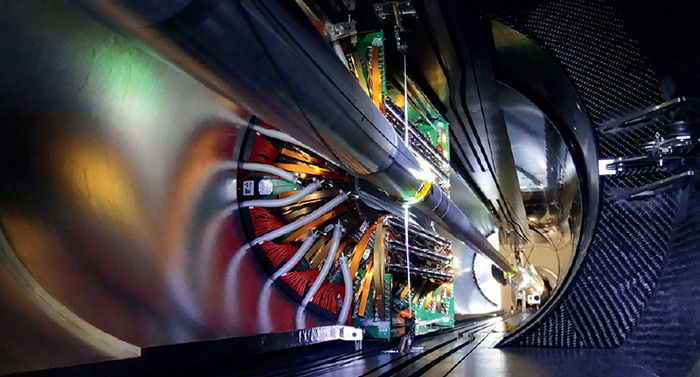
\includegraphics[width=\textwidth]{2_ExperimentalSetup/Figures/cmspixel}
  		\caption{The pixel barrel being re-installed after the Long Shutdown in 2015, around the beam pipe at CMS~\cite{Christine:2024986}}
  		\label{fig:pix}
  	\end{minipage}
  	\hfill
  	\begin{minipage}[t]{0.4\textwidth}
  		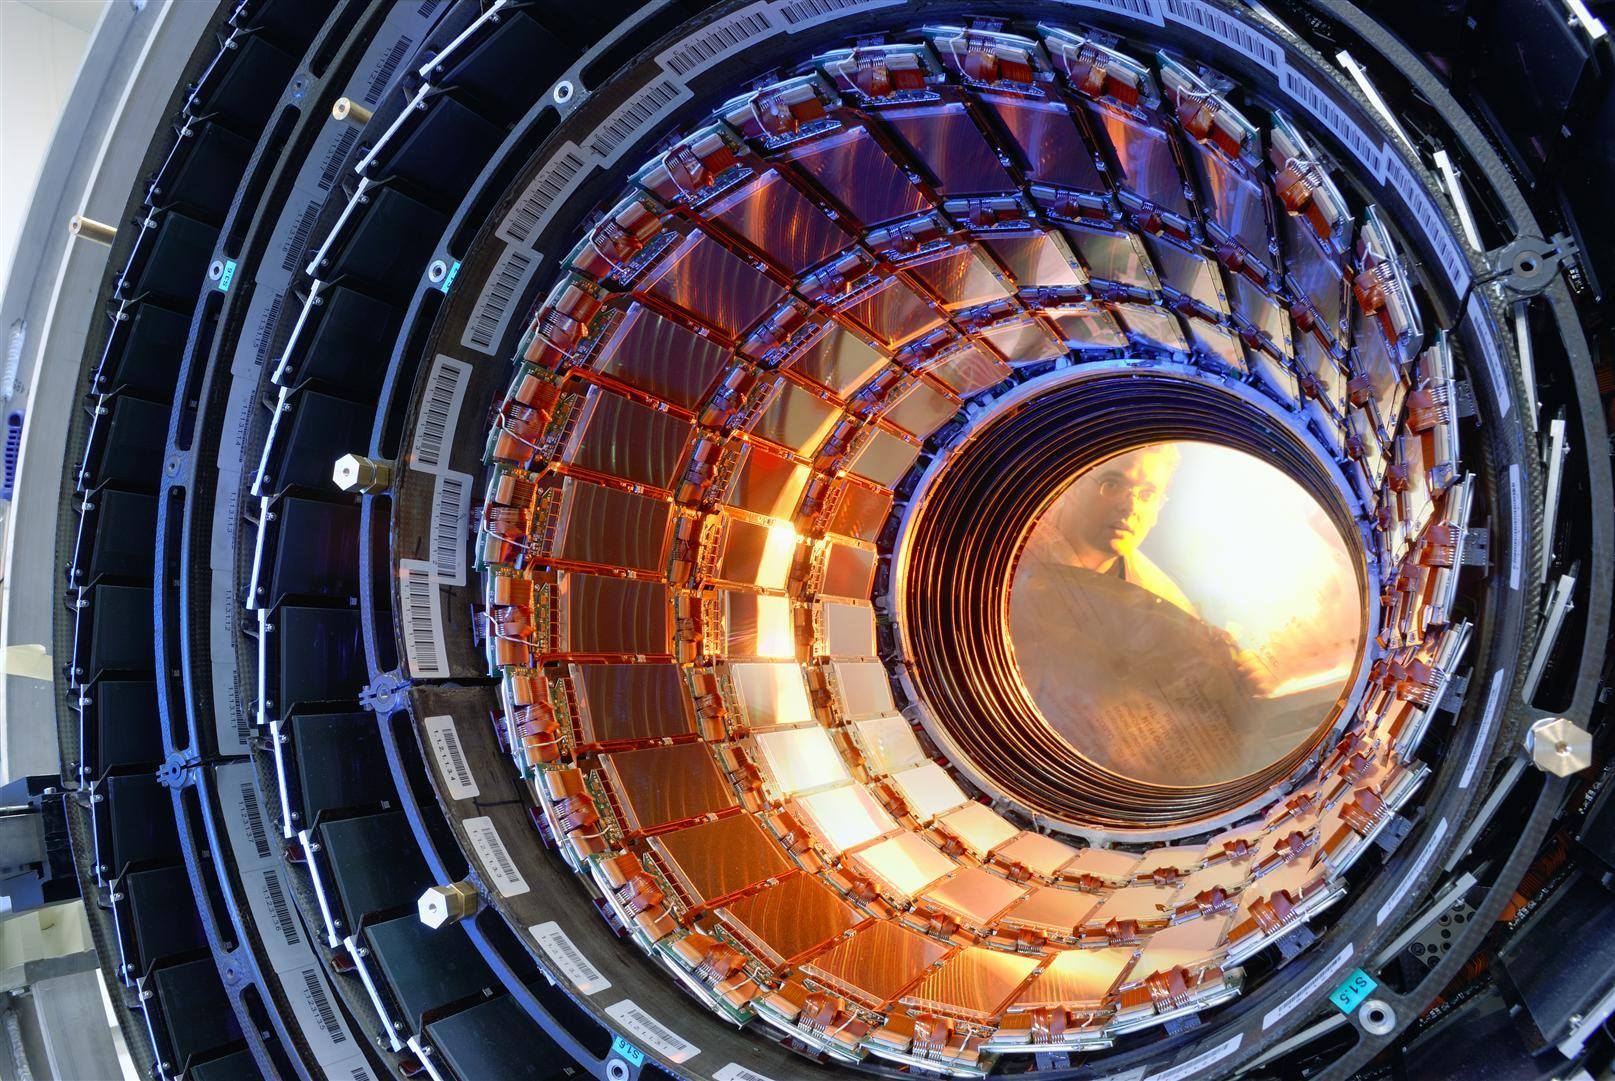
\includegraphics[width=\textwidth]{2_ExperimentalSetup/Figures/cmsbarrel}
  		\caption{First half of the inner tracker barrel, consisting of three layers of silicon modules~\cite{beautiful:1998635}.}
  			\label{fig:Trackpics}
  	\end{minipage}
  
  	%	(from https://twiki.cern.ch/twiki/bin/view/CMSPublic/LumiPublicResults#Online_Luminosity_AN2 )
  \end{figure}
  
  
  
  
  
\subsection{Data acquisition}
\label{sec:DAQ}
% event display https://cds.cern.ch/record/2242076/files/DP2017_001.pdf
At a design luminosity of 10$^{34}$ \si{ \per \square \meter \per \second}, the proton interaction rate exceeds 1 \si{ \giga \hertz}. This makes it impossible for the CMS experiment to store all the data generated. For this, a two level trigger system has been put in place. The first level (Level-1) is a custom hardware system, while a second level (HLT) is software based running on a large farm of computers. 
In run II, with the increase in centre of mass energy and a higher luminosity, a larger number of simultaneous inelastic collisions per crossing is expected with respect to run I. For this, the CMS Level-1 has been upgraded~\cite{1748-0221-12-03-C03021}. 

\subsubsection*{CMS Level-1 trigger}
The Level-1 trigger has to be a flexible, maintainable system, capable of adapting to the evolving physics programme of CMS~\cite{Khachatryan:2016bia}. Its output rate is restricted to 100 \si{ \kilo \hertz} imposed by the CMS readout electronics. It is implemented by custom hardware and selects events containing candidate objects - eg ionization deposits consistent with a muon, or energy clusters corresponding to an electron / photon / tau lepton / missing transverse energy / jet. Collisions with large momenta can be selected by using scalar sum of the transverse momenta of the jets. 

\begin{comment}
\begin{figure}[h]
	\centering
	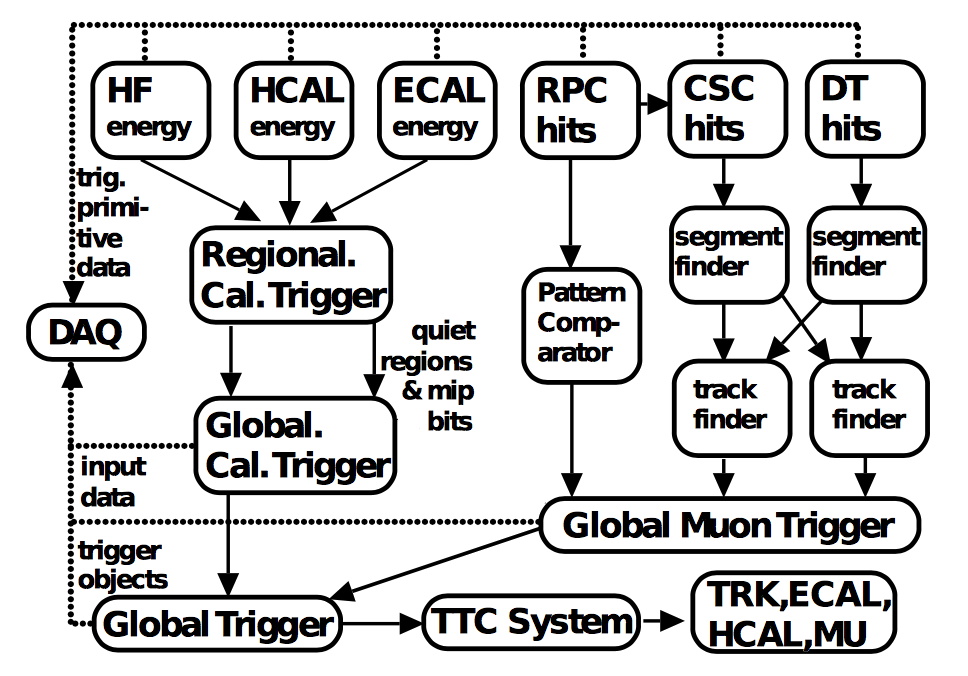
\includegraphics[width=0.5\linewidth]{2_ExperimentalSetup/Figures/imageedit_13_6388071145}
	\caption{The CMS level 1 trigger system for run I. Data from the calorimeters are processed regionally (RCT) ad the globally (GCT). Data from the muon chambers are processed via a global muon trigger (GMT). A global trigger (GT) combines the GCT and GMT, making a trigger decision. Th data acquisition system (DAQ) reads data from the tracker (TRK) via the trigger, timing  and control (TTC) system \cite{Khachatryan:2016bia}.}
	\label{fig:level1}
\end{figure}
\end{comment}

By buffering the raw data from the CMS subdetectors in front-end drivers, the level-1 trigger has a pipeline memory of 3.2 \si{ \micro \second} to decide whether to keep an event or reject it. 
%In \fig{fig:level1} the structure of the trigger is shown. 
The trigger primitives (TP) from the calorimeters and muon detectors are processed in several steps and combined into a global trigger. This information is then combined with the input from the other subsystems for the HLT. The separate inputs are synchronized to each other and the LHC orbit clock and sent to the global trigger module. Here, level-1 trigger algorithms are performed within 1 \si{ \micro \second} to decide whether to  keep the event. 

For run II, all hardware, software, databases and the timing control system have been replaced. The main changes are that the muon system now uses the redundancy of three muon detector system earlier to make a high resolution muon trigger. Other upgrades are that the calorimeter system isn't bound any more for streaming data the data and the global trigger has more level-1 trigger algorithms. 
% see https://indico.cern.ch/event/432527/contributions/1072399/attachments/1320545/1980311/ichep2016.pdf

\subsubsection*{CMS HLT trigger}
The HLT is an array of commercially available computers with programmable menu that has output rate of on average 400 \si{ \hertz} for off-line event storage.
The data processing is based on a HLT path. This is a  set of algorithmic steps to reconstruct objects and make selections on them.  Here, the information of all sub detectors can be used to perform algorithms on higher level reconstructed objects. 
%(FIXME: tracker in hlt or already in L1? )

\subsection{Phase 1 upgrades}
\label{sec:Phase1}
Before the start of taking collision data for 13~\TeV\ operations on 3 June 2015, CMS had a long shutdown (LS1)\cite{Pralavorio:2024977}. During this shutdown, the section of the beryllium beam pipe within CMS was replaced by a narrower one. This operation required the pixel to be  removed and reinserted into CMS. In Run 2, higher particle fluxes with respect to Run 1 are expected. To avoid long damage caused by the intense particle flux at the heart of CMS, the tracker is been made ready to operate at much lower temperature than during Run I.  The electromagnetic calorimeter preshower system had been damaged during Run 1, therefore the preshower discs were removed, repaired and reinstalled successfully inside CMS in 2014. To help the discrimination between interesting low momentum muons coming from collisions and muons caused by backgrounds, a fourth triggering and measurement station for muons was added in each of the end caps. Several new detectors were installed into CMS for measuring the collision rate within the detector and monitors beam related backgrounds. 

During the LS1, the  muon system underwent major upgrades~\cite{Guiducci:1966038,Battilana:2239185}. In the fourth station of each end cap, the outermost rings of CSC and RPC chambers were completed, providing an angular coverage of $1.2<$ \abspsrap $<1.8$ for Run 2, increasing the system redundancy, and allowing tighter cuts on the trigger quality. In order to reduce the environmental noise, outer yoke discs have been placed on both sides for the end caps. 
At the innermost rings of the first station, the CSCs have been upgraded by refurbishing the readout electronics to make use of the full detector granularity instead of groups of three as was the case for Run 1. In \fig{fig:muonsys} (right), the refurbishing of the CSCs is shown.
% also see https://indico.cern.ch/event/308134/sessions/59604/attachments/588148/809429/Lecture.pdf

Since thee HF experiences intense particle fluxes, it became clear during Run 1 that the glass windows of the PMTs need replacing. For the ECAL in Run 1, the energy reconstruction happened  via a weighted sum of the digitized samples~\cite{Chatrchyan:2013dga}. For Run 2 however, the reconstruction had to be made more resistant for out of time pile up and a multi-fit approach has been set into place. In this approach, the pulse shape is modelled as a sum of one in-time pulse plus the out of time pulses \cite{1748-0221-12-01-C01069}. The energy resolution is better than 2\%  in the central barrel region and 2-5 \% elsewhere.
% https://indico.cern.ch/event/477407/contributions/2305075/attachments/1368970/2075215/hc16-edm.pdf
% see http://iopscience.iop.org/article/10.1088/1748-0221/12/01/C01069/pdf at vub
% http://www.bo.infn.it/sminiato/sm16/03_Mercoledi/Sera/08_Brianza.pdf
% https://indico.cern.ch/event/472938/contributions/1150724/attachments/1273518/1888397/ECALEnergyOverview_CALOR.pdf
%https://inspirehep.net/record/1344855/files/10.1088_1742-6596_587_1_012001.pdf

 During the first data taking period of the LHC (2010 to 2013), the tracker operated at +4\si{ \degree C}. With the higher LHC beam intensities from 2015 onwards, the tracker needs to be operated at much lower temperatures. This is due to the fact with intense irradiation, the doping concentration changes, the leakage current increases proportional to the fluence and the charge collection efficiency decreases due to charge trapping. Mostly the leakage current (I) is affected by the temperature change: 
\begin{equation}
I \propto T^2 e^{-\frac{E_g}{2kT}}, 
\end{equation}
where $T$ is the operating temperature, $E_g$ the band gap and $k$ the Boltzmann constant. There is approximately a factor 15 between the leakage currents at room temperatures and at $-10$ \si{ \degree C}. 
% see http://www.hephy.at/user/friedl/diss/html/node14.html

During the LS1, the CMS cooling plant was refurbished\cite{running:1998606}(\fig{fig:TrackLS1}) and the fluorocarbon cooling system overhauled. To help to suppress the humidity inside the tracker, new methods for vapour sealing and insulation were applied (\fig{fig:TrackLS11}. Furthermore, several hundred high-precision sensors are used to monitor the humidity and temperature. In order to get as dry air as possible, a new dry-gas plant provides eight times more dry gas (air or nitrogen) than during the first run, and allows regulation if the flow. As final addition, the cooling bundles outside the tracker are equipped with heater wires and temperature sensors in order to maintain safe operations above the cavern dew point For the data taking in 2015-2016, the tracker operated at $-15$\si{ \degree C}.

\begin{figure}[htbp]
	\centering
	\begin{minipage}[t]{0.4\textwidth}
		%	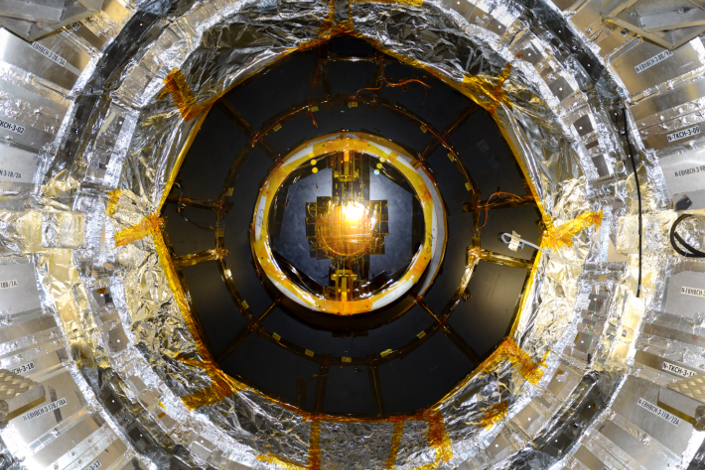
\includegraphics[width=\textwidth]{2_ExperimentalSetup/Figures/Tracker_bulkhead}
		\includegraphics[width=\textwidth]{2_ExperimentalSetup/Figures/BHIsis}
		\caption{Tracker bulkhead being put into closed state with insulation pieces installed during an early trial in fall 2013}
		\label{fig:TrackLS11}
	\end{minipage}
	\hfill
	\begin{minipage}[t]{0.59\textwidth}
		%		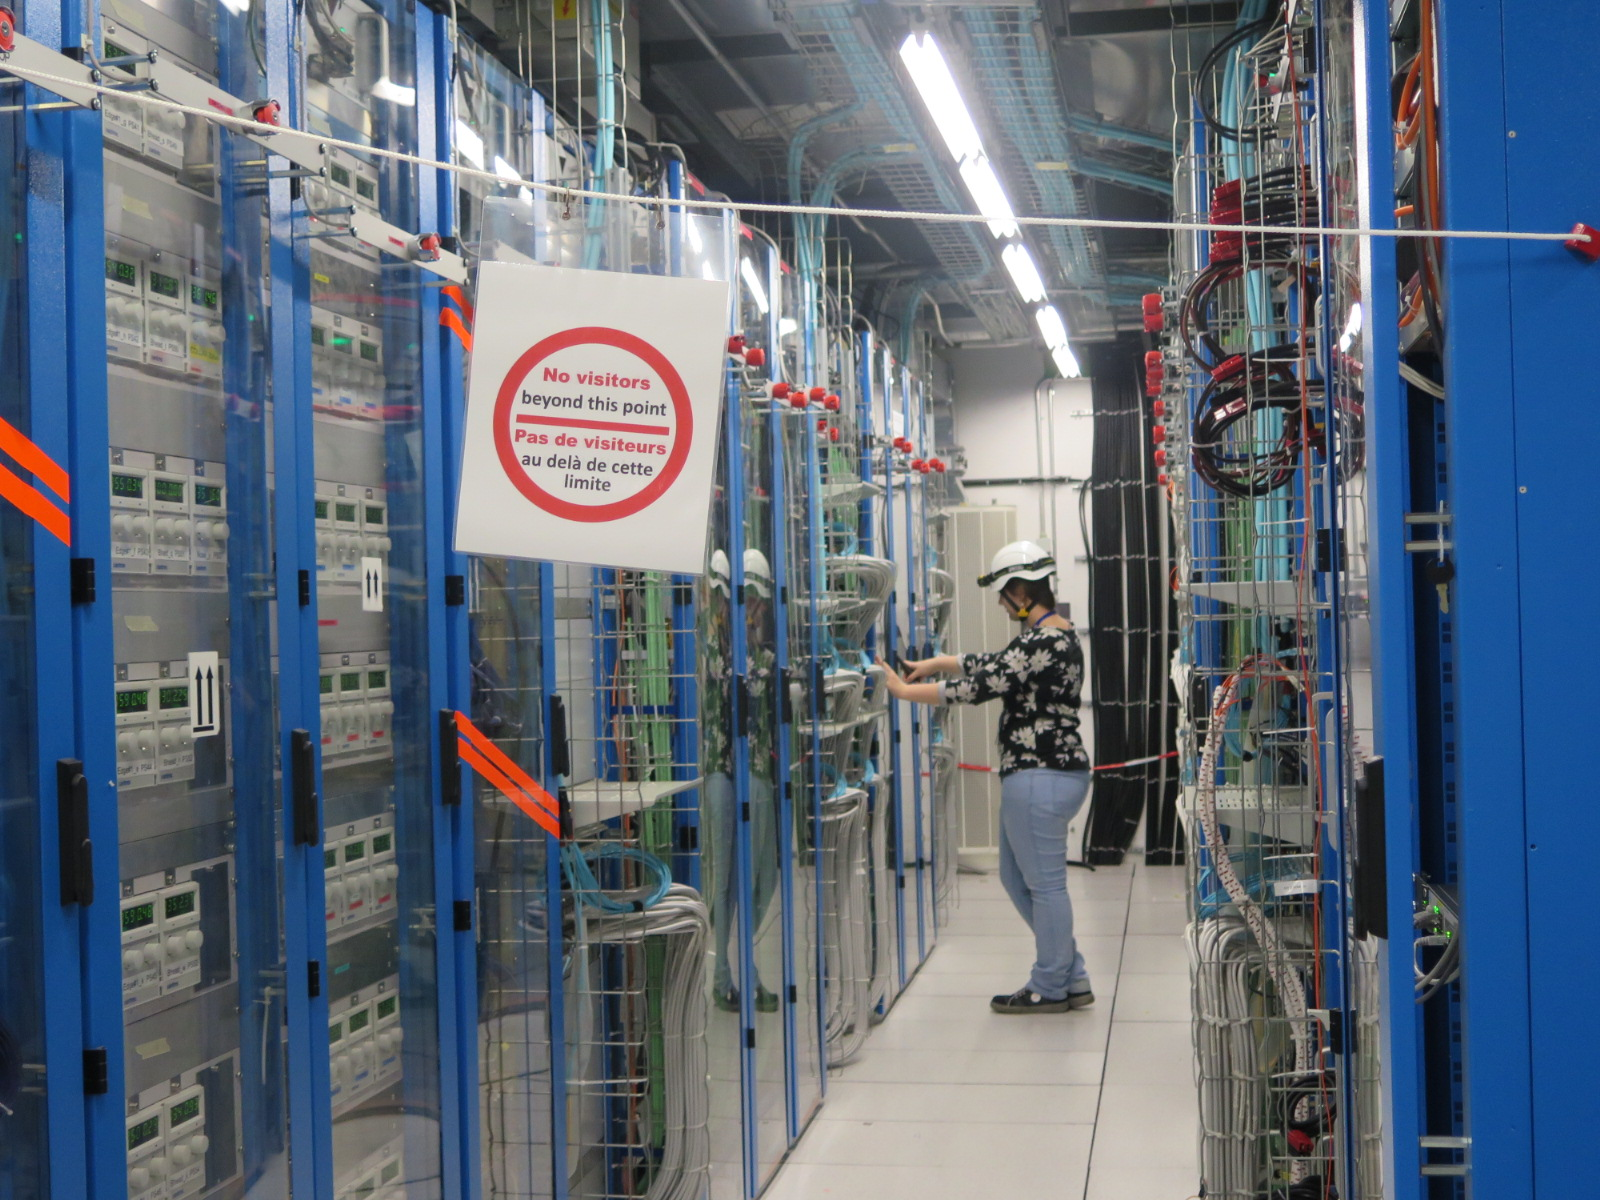
\includegraphics[width=\textwidth]{2_ExperimentalSetup/Figures/IMG_0138}
		%	\caption{Tracker service racks containing the electronics coming from the tracking systems.}
		
		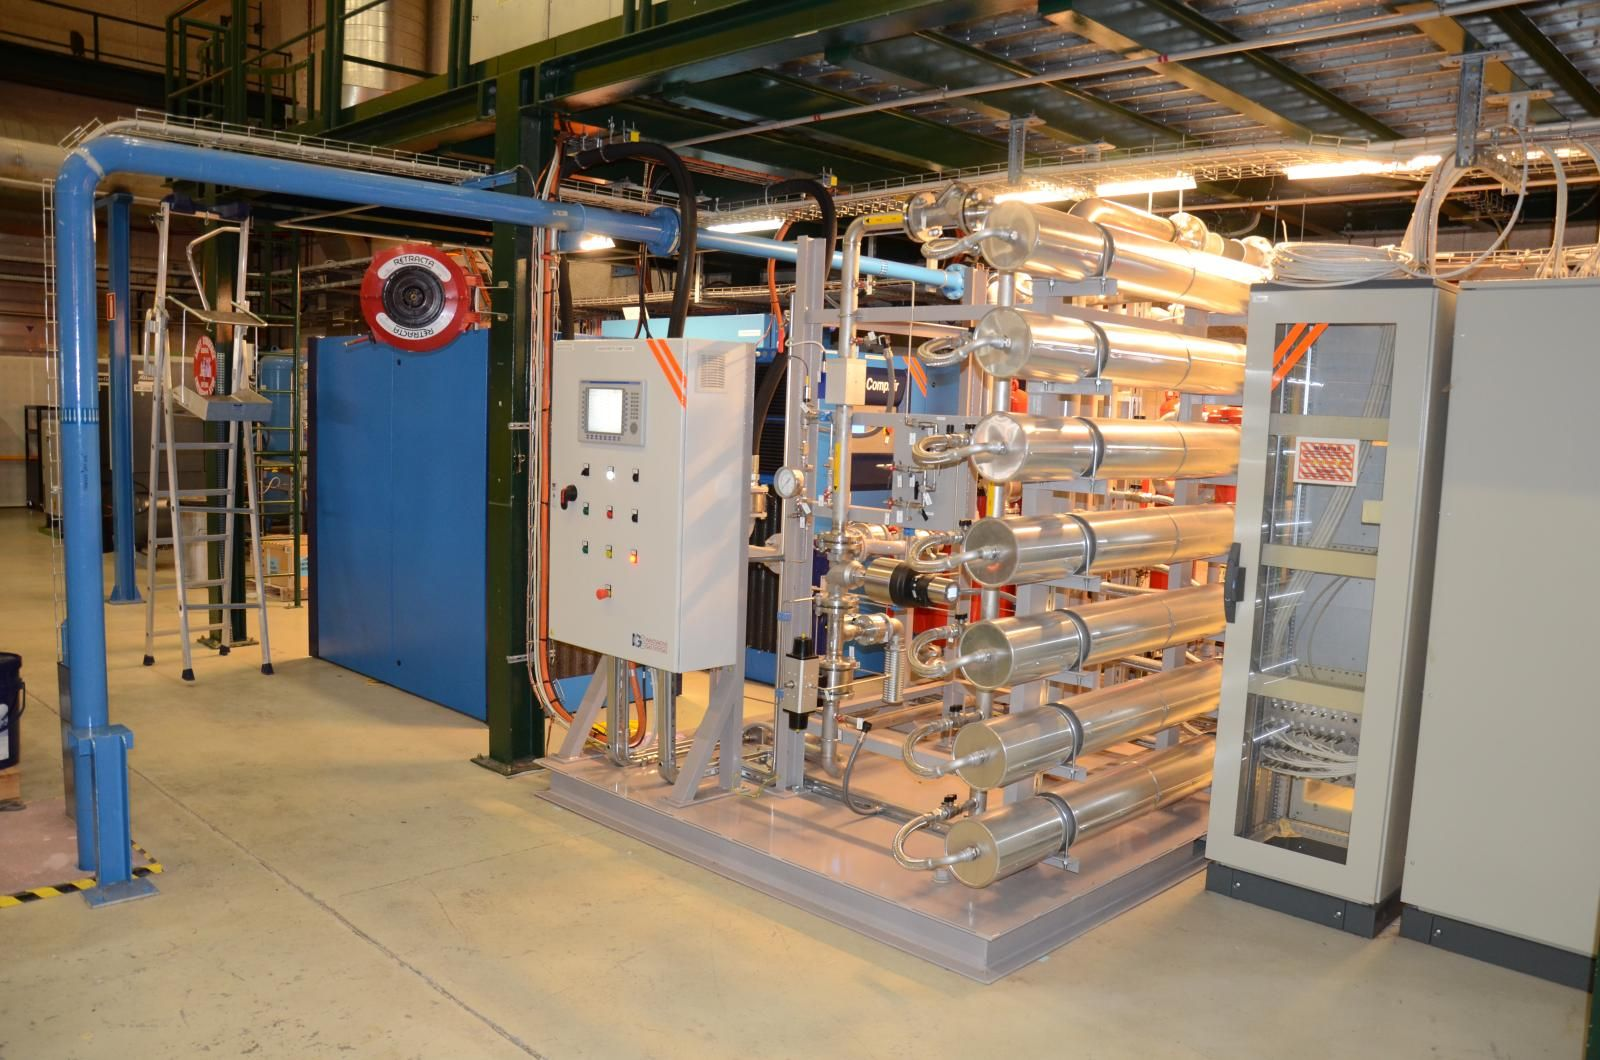
\includegraphics[width=\textwidth]{2_ExperimentalSetup/Figures/plant}
		\caption{New Tracker high-capacity dry-gas plant with membrane separation system~\cite{Pralavorio:2024977}.}
		\label{fig:TrackLS1}
	\end{minipage}
	
	%	(from https://twiki.cern.ch/twiki/bin/view/CMSPublic/LumiPublicResults#Online_Luminosity_AN2 )
\end{figure}


After the first half of Run 2, the innermost part of detection material in CMS (pixel) was upgraded by adding a fourth layer , enhancing the particle tracking capabilities of CMS. The data used in the framework of this thesis however is from before this upgrade. 


\subsection{CMS computing model}
The selected data is stored, processed and dispersed via the Worldwide Large Hadron Collider GRID (WLCG)\cite{Grandi:814248,Eck:840543}. This has a tiered structure that function as a single, coherent system:. 

At CERN, a single Tier-0 is located. The raw data collected by CMS is archived here, and a first reconstruction of the data is done. This data is then already in a file format usable for physics analysis. Furthermore, it is able to reprocess data when new calibrations are made available. The Tier-0 site distributes this data to a total of seven Tier-1 centres. They carry out data reprocessing and store real data as well as simulated  data. The Tier-1 further distribute the data to over 50 Tier-2 centres. These make the data accessible for physics analysis and are also being used for the production of simulated data. The data is made accessible for  physicists around the world. 
